\documentclass{article}
\usepackage[english]{babel}

\usepackage{graphicx}

\title{Final Project}
\author{Jackson Blake and Allen Braun}

\begin{document}
\maketitle
\section{Introduction}
We create a swamp cooler using an Arduino attached to a circuit. The circuit continually measures temperature and humidity of the cooler. It uses the values of these measurements to switch between four states of running, idle, disabled, and error. The swamp cooler reacts to these states, and activates a fan and parts as needed to maintain certain temperature and humidity.\\
\section{Components}
Part DS1307, Real time clock module: Keeps track of time even when unpowered. It is also used to give an exact timestamp for state and vent changes\\
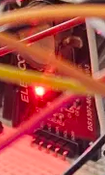
\includegraphics[height=40mm]{realtimeclock.png}\\
28BYJ-48, Stepper motor: Moves in precise programmable increments. Used as a stand in for an "adjustable vent"\\
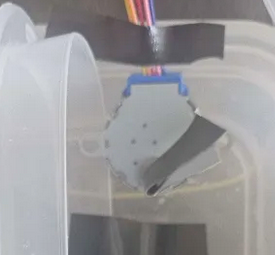
\includegraphics[height=40mm]{steppermotor.png}\\
ULN2003, Stepper motor driver: Acts as a power adapter, and intermediary between the board and the 28BYJ-48\\
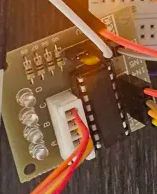
\includegraphics[height=40mm]{steppermotordriver.png}\\
Generic, Breadboard power supply module: Separate power supply that connects to the edge of a breadboard. Supplies more power than the arduino so it can safely run motors without frying\\
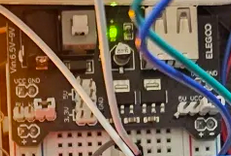
\includegraphics[height=40mm]{breadboardpower.png}\\
Generic, DC Motor: No fine control, spin direction is just based on what end is power, which is ground, speed is based on voltage pulsing. Used in our project to power the fan for when things get hot\\
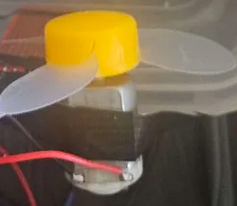
\includegraphics[height=40mm]{dcmotor.png}\newpage
L293D, motor driver: Acts as a power supply and direction controller for 1 to 4 motors. In our case just used to drive the DC motor either on or off\\
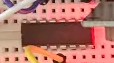
\includegraphics[height=40mm]{motordriver.png}\\
LCD1602, 16x2 LCD display: Used to display the temperature and humidity while the cooler is working normally. Displays the reason why it is not working normally if it is not\\
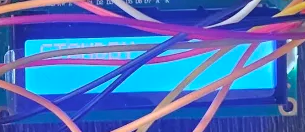
\includegraphics[height=40mm]{lcd.png}\\
DHT11, humidity and temperature sensor: Gives digital output over 1 wire for humidity and temperature in percentage and celsius respectively, doesn't need any outside conversion\\
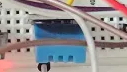
\includegraphics[height=40mm]{humidtemp.png}\newpage
Water level sensor: Detects water on it, outputs a unitless analog signal so needs some calibration/trial error to set the level on it\\
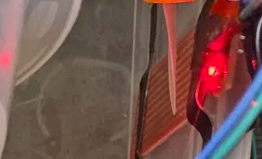
\includegraphics[height=40mm]{waterlevel.png}\\
3x push buttons: Used to trigger the interrupts that switch between states\\

\includegraphics[height=30mm]{pushbutton.png}\\
4x LEDs (yellow/green/blue/red): Used to show the disabled, idle, fan running, and low-water-error states respectively\\
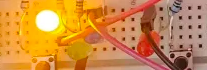
\includegraphics[height=40mm]{leds.png}\\
Potentiometer: Used to adjust the contrast on the LCD and make it readable\\

\includegraphics[height=30mm]{potentiometer.png}\newpage
7x 100 ohm resistors: Used as pulldowns for the buttons and protection for the LEDs\\
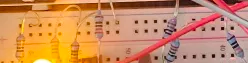
\includegraphics[height=30mm]{ohmresistors.png}\\
\section{System Overview}
The code for the system is based off of a main loop that keeps track of states and executes code as needed. 
At the beginning of the loop, it checks if a state has changed, and outputs this into the serial monitor. If the vent position is toggled, it also displays this to the serial monitor.\\
When the state is changed to disabled, the yellow LED turns on, and the fan turns off. The LCD also prints standby.\\
When the state is changed to idle, the green LED turns on, it reads the temperature and water level, displays this to the LCD.\\
If the temperature is too high, the state is changed to running. If the water is too low, the state is changed to error.\\
When the state is changed to error, the red LED turns on, it turns off the fan, and displays an error message.
When the state is changed to running, the blue LED turns on, the fan is turned on, and readings gets sent to the LCD.\\
If the temperature is too low, it sets the state to idle. If the water gets too low, the state is changed to error.\\
\section{Circuit}
We obtain the following image of the final circuit:\\
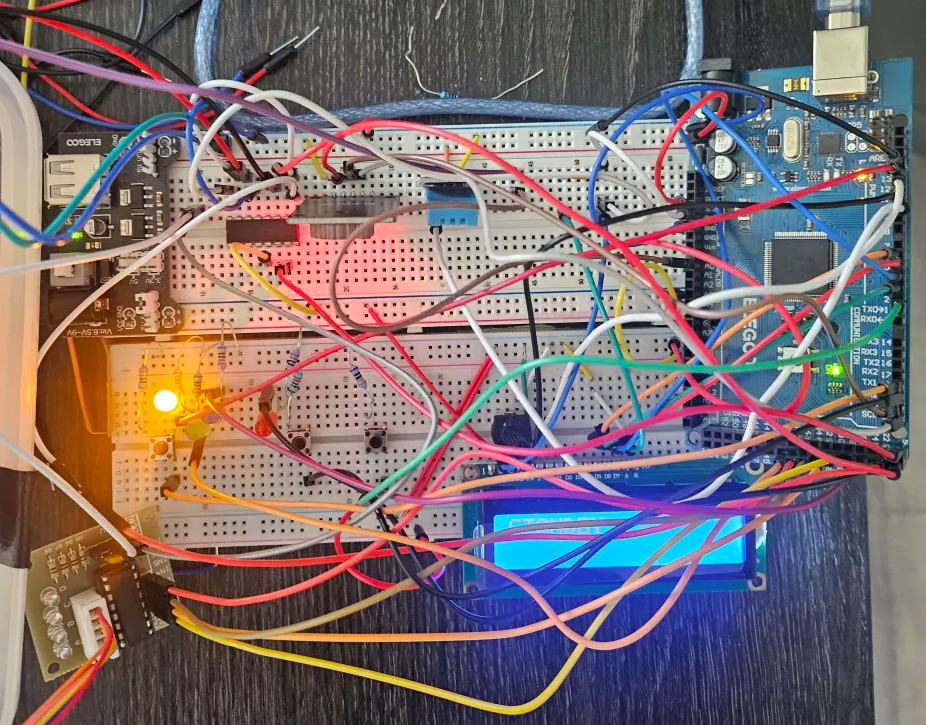
\includegraphics[height=100mm]{circuit.png}
\section{Schematic}
A schematic diagram for the circuit is found to be as follows:\\
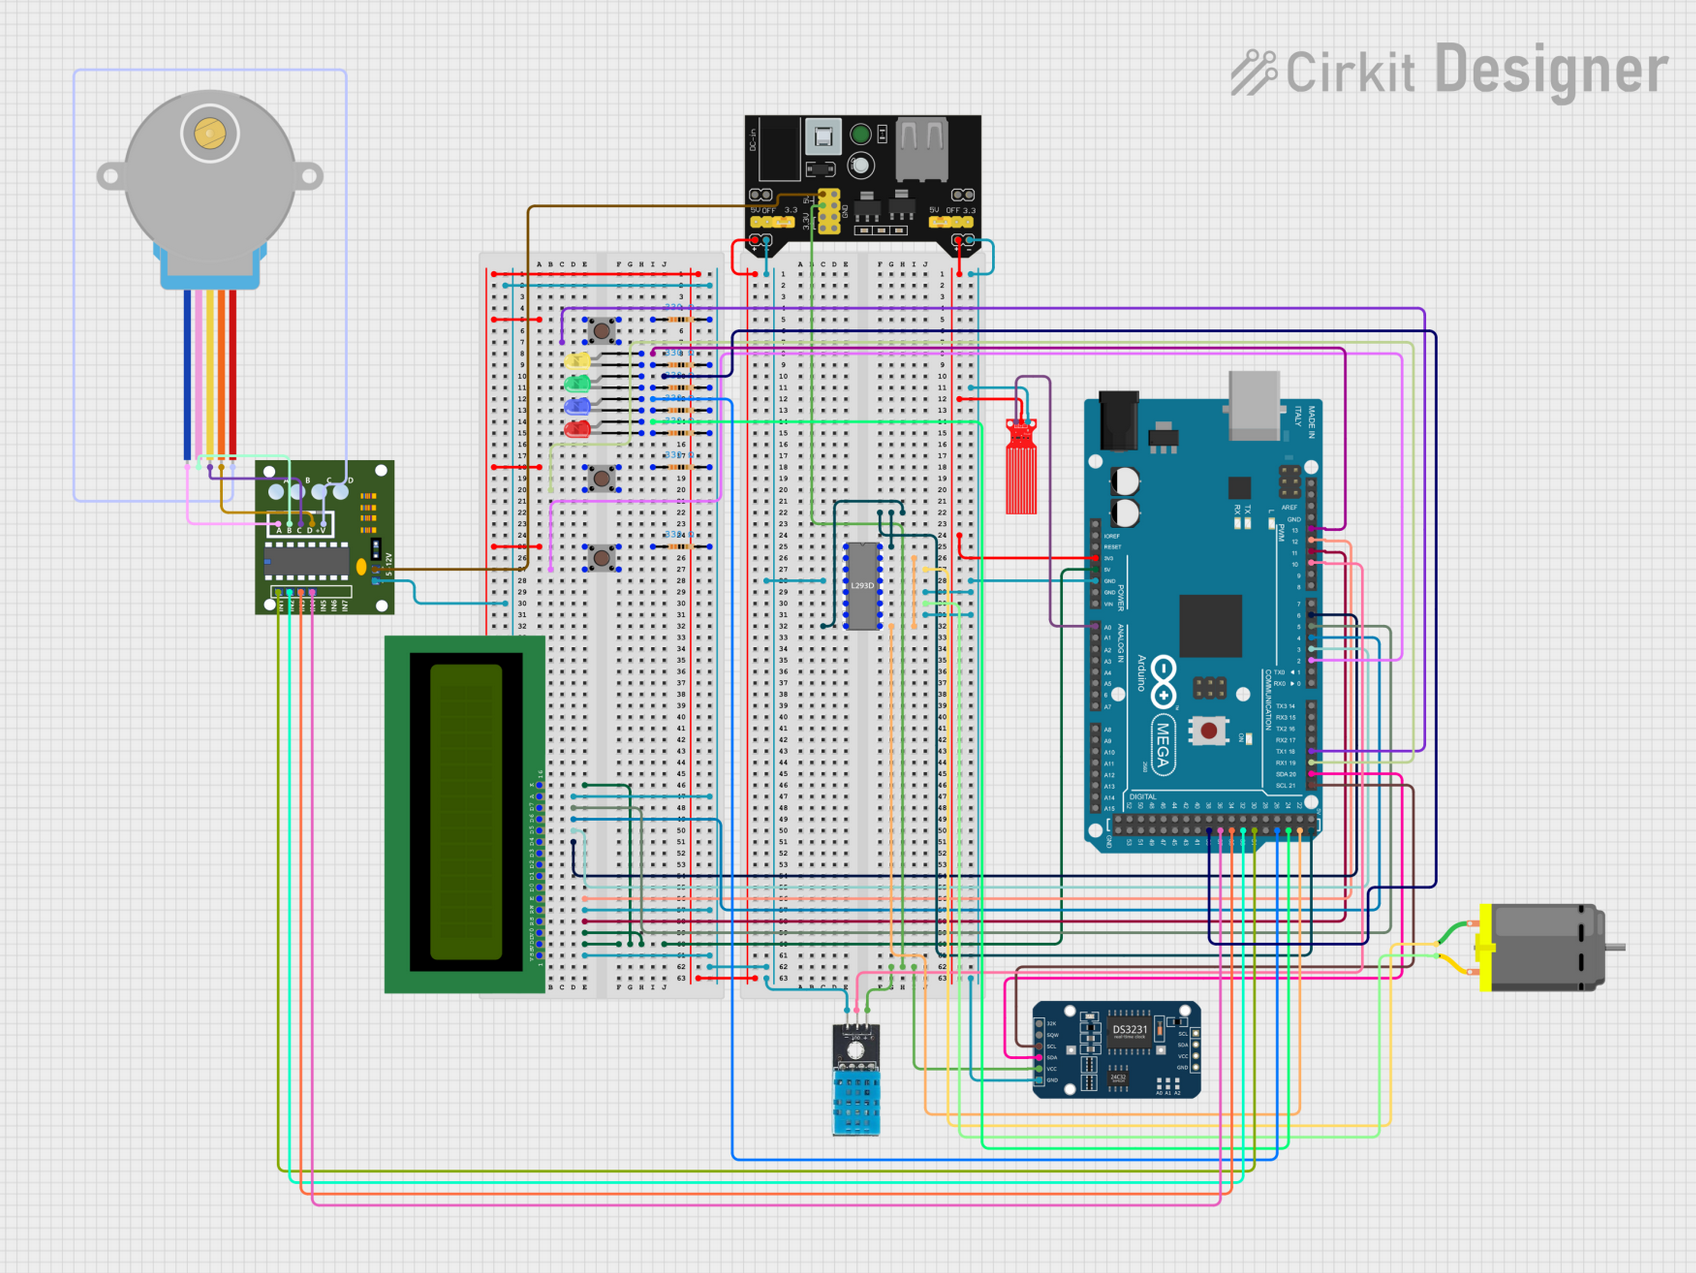
\includegraphics[height=100mm]{schematic.png}
\section{Video Demonstration}
A video demonstration can be found on youtube here:\\
https://www.youtube.com/watch?v=EpjEM92hOkA\\
For further information, see the github:\\
https://github.com/dignitydignity/CPE-301-finalproject
\end{document}